\documentclass[aspectratio=169,11pt]{beamer}
\def\courseweek{5}
% Shared style for the Introduction to Information Geometry lecture slides.
% Compile the lecture .tex files from this directory.
\providecommand{\courseweek}{1}
\usepackage[T1]{fontenc}
\usepackage[utf8]{inputenc}
\usepackage[sc]{mathpazo}
\renewcommand{\sfdefault}{lmss}
\renewcommand{\ttdefault}{lmtt}
\usepackage{amsmath,amssymb,mathtools}
\usepackage{tikz}
\usetikzlibrary{arrows.meta,calc,positioning}
\usepackage{pgfplots}
\pgfplotsset{compat=1.18}
\usepackage{booktabs}

\definecolor{courseink}{HTML}{173749}
\definecolor{coursemuted}{HTML}{526674}
\definecolor{courseteal}{HTML}{0E7287}
\definecolor{coursecopper}{HTML}{B66B43}
\definecolor{courseline}{HTML}{D4E0E3}
\definecolor{coursepale}{HTML}{EFF5F5}

\setbeamercolor{normal text}{fg=courseink,bg=white}
\setbeamercolor{structure}{fg=courseteal}
\setbeamercolor{frametitle}{fg=courseink,bg=white}
\setbeamercolor{title}{fg=courseink}
\setbeamercolor{subtitle}{fg=coursemuted}
\setbeamercolor{block title}{fg=courseink,bg=white}
\setbeamercolor{block body}{fg=courseink,bg=white}
\setbeamercolor{alerted text}{fg=coursecopper}
\setbeamerfont{title}{family=\rmfamily,series=\bfseries,size=\fontsize{32}{37}}
\setbeamerfont{frametitle}{family=\rmfamily,series=\bfseries,size=\fontsize{26}{31}}
\setbeamerfont{normal text}{size=\fontsize{18}{22}}
\setbeamerfont{subtitle}{size=\fontsize{17}{21}}
\setbeamersize{text margin left=0.78cm,text margin right=0.78cm}
\setbeamertemplate{navigation symbols}{}
\setbeamertemplate{itemize items}[circle]
\setbeamertemplate{enumerate items}[default]
\setbeamertemplate{blocks}[default]
\setlength{\parskip}{0.22em}
\setbeamertemplate{footline}{%
  \leavevmode\hbox to \paperwidth{\hspace{.78cm}%
  {\color{coursemuted}\fontsize{8.5}{10}\selectfont Introduction to Information Geometry \hspace{.32cm} / \hspace{.32cm} Week \courseweek}%
  \hfill{\color{coursemuted}\fontsize{8.5}{10}\selectfont \insertframenumber\hspace{.17cm}/\hspace{.17cm}\inserttotalframenumber}\hspace{.78cm}}%
  \vskip.17cm
}
\setbeamertemplate{frametitle}{%
  \vspace{.13cm}
  \insertframetitle\par
  \vspace{.08cm}
}
\setbeamertemplate{title page}{%
  \vspace*{1.00cm}
  {\color{courseteal}\fontsize{10}{13}\selectfont\bfseries
  INTRODUCTION TO INFORMATION GEOMETRY\par}
  \vspace{.40cm}
  {\usebeamerfont{title}\usebeamercolor[fg]{title}\inserttitle\par}
  \vspace{.22cm}
  {\usebeamerfont{subtitle}\usebeamercolor[fg]{subtitle}\insertsubtitle\par}
  \vfill
  {\color{coursemuted}\fontsize{13}{16}\selectfont Christopher Lee\par}
  \vspace{.34cm}
}

\pgfplotsset{
  courseplot/.style={
    width=11.05cm,
    height=5.15cm,
    axis line style={coursemuted!75},
    tick style={coursemuted!65},
    ticklabel style={font=\scriptsize,color=coursemuted},
    label style={font=\normalsize,color=courseink},
    grid=major,
    major grid style={courseline!70,line width=.4pt},
    line width=1.45pt,
    legend style={font=\small,draw=none,fill=none,at={(.98,.03)},anchor=south east},
    clip=true
  }
}

\newcommand{\highlightmath}[1]{{\color{courseteal}#1}}
\newcommand{\thinrule}{\par\vspace{.25cm}{\color{courseline}\rule{\linewidth}{.8pt}}\par}

% A one-dimensional state space.  x=0 and x=1 are placed at 0 and 9 units.
\newcommand{\stateinterval}[1]{%
 \begin{tikzpicture}[x=1cm,y=1cm]
   \draw[courseink,line width=1.25pt] (0,0)--(9,0);
   \foreach \pos/\lab in {0/0,9/1} {
     \fill[courseink] (\pos,0) circle(2.7pt);
     \node[below=9pt,text=coursemuted] at (\pos,0) {\(\lab\)};
   }
   #1
 \end{tikzpicture}%
}

% Paired pages are separate frames in the PDF, with matching titles.
% Supply the whole frame body for each version; the instructor may edit them
% independently without changing overlay logic.
\newcommand{\coursepair}[3]{%
  \begin{frame}{#1}#2\end{frame}%
  \begin{frame}{#1}#3\end{frame}%
}

% Equilateral representation of the categorical simplex, in barycentric
% coordinates with vertices A=(0,0), B=(1,0), C=(1/2,sqrt(3)/2).
\newcommand{\coursesimplex}[1]{%
 \begin{tikzpicture}[scale=4.9]
  \fill[coursepale] (0,0)--(1,0)--(.5,.8660254)--cycle;
  \draw[courseink,line width=.65pt] (0,0)--(1,0)--(.5,.8660254)--cycle;
  \node[below left,font=\small] at (0,0) {A};
  \node[below right,font=\small] at (1,0) {B};
  \node[above,font=\small] at (.5,.8660254) {C};
  #1
 \end{tikzpicture}%
}

\title{Surprisal and Shannon Entropy}
\subtitle{Week 5 \(\cdot\) Lecture 1}
\date{}
\begin{document}
\begin{frame}[plain]\titlepage\end{frame}

\begin{frame}{The information in one outcome}
An outcome with probability \(p\) has surprisal
\[
\highlightmath{I(p)=-\log_2 p}\quad\text{bits}.
\]
\vspace{.45cm}
With natural logarithms, \(-\ln p\) measures surprisal in nats.
\vspace{.47cm}
An outcome assigned a smaller probability carries greater surprisal
when it occurs.
\end{frame}

\begin{frame}{Surprisal changes nonlinearly}
\vspace{-.18cm}
\begin{center}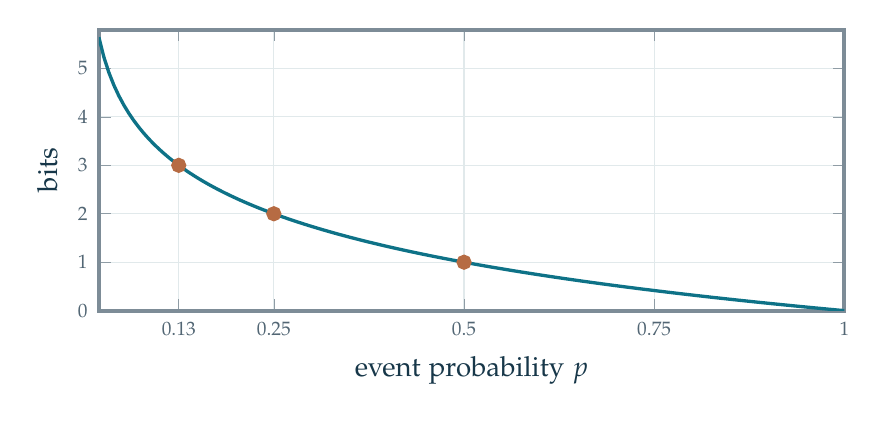
\begin{tikzpicture}
\begin{axis}[courseplot,xmin=.02,xmax=1,ymin=0,ymax=5.8,
 xlabel={event probability $p$},ylabel={bits},xtick={.125,.25,.5,.75,1},
 ytick={0,1,2,3,4,5}]
\addplot[courseteal,very thick,domain=.02:1,samples=150]{-ln(x)/ln(2)};
\addplot[only marks,coursecopper,mark=*,mark size=2pt]
coordinates{(.125,3)(.25,2)(.5,1)};
\end{axis}\end{tikzpicture}\end{center}
\vspace{-.1cm}
Halving a probability increases surprisal by exactly one bit.
\end{frame}

\coursepair{Computing surprisal}{
An event has probability \(p=\frac18\).
\vspace{.55cm}
Find its surprisal in bits and in nats:
\[
I_2=-\log_2(\tfrac18)=\;?,
\qquad I_e=-\ln(\tfrac18)=\;?.
\]
}{
An event has probability \(p=\frac18\).
\vspace{.55cm}
Its surprisal in bits and in nats is
\[
\highlightmath{I_2=3}\text{ bits},
\qquad \highlightmath{I_e=\ln8}\text{ nats}.
\]
}

\begin{frame}{Entropy is average surprisal}
For a categorical law \(P=(p_1,\ldots,p_n)\),
\[
\highlightmath{H(P)=-\sum_i p_i\log_2 p_i}\quad\text{bits}.
\]
\vspace{.50cm}
This is the expected information of one random draw.
\vspace{.37cm}
The convention \(0\log 0=0\) makes entropy continuous
at the boundary of a finite simplex.
\end{frame}

\coursepair{Entropy of a three-outcome law}{
Let \(P=(\frac12,\frac14,\frac14)\).
\vspace{.4cm}
Evaluate
\[
H(P)=-\frac12\log_2\frac12
-\frac14\log_2\frac14
-\frac14\log_2\frac14.
\]
\vspace{.4cm}
Find \(H(P)\) in bits.
}{
Let \(P=(\frac12,\frac14,\frac14)\).
\vspace{.4cm}
The three terms are \(\frac12,\frac12,\frac12\) bits.
\vspace{.32cm}
\[
\highlightmath{H(P)=\frac32}\text{ bits}.
\]
\vspace{.32cm}
The uniform three-outcome law has a larger entropy, \(\log_2 3\).
}

\begin{frame}{Binary entropy}
For \(P_p=(p,1-p)\),
\[
\highlightmath{h(p)=-p\log_2p-(1-p)\log_2(1-p)}.
\]
\vspace{.35cm}
\begin{center}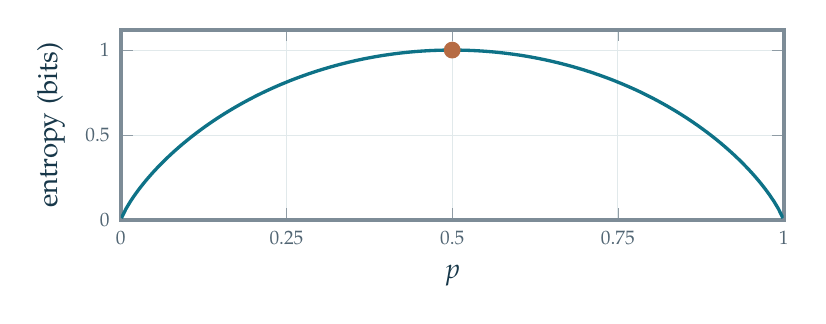
\begin{tikzpicture}
\begin{axis}[courseplot,width=10cm,height=4cm,xmin=0,xmax=1,
 ymin=0,ymax=1.12,xlabel={$p$},ylabel={entropy (bits)},
 xtick={0,.25,.5,.75,1},ytick={0,.5,1}]
\addplot[courseteal,very thick,domain=.001:.999,samples=150]
{-x*ln(x)/ln(2)-(1-x)*ln(1-x)/ln(2)};
\addplot[only marks,coursecopper,mark=*,mark size=2.3pt]coordinates{(.5,1)};
\end{axis}\end{tikzpicture}\end{center}
\end{frame}

\coursepair{Where is binary entropy greatest?}{
Using natural logs, let
\[
h(p)=-p\ln p-(1-p)\ln(1-p).
\]
\vspace{.35cm}
Compute \(h'(p)\), solve \(h'(p)=0\), and check concavity.
\vspace{.3cm}
\[
h'(p)=\;?,\qquad h''(p)=\;?.
\]
}{
Using natural logs, let
\[
h(p)=-p\ln p-(1-p)\ln(1-p).
\]
\vspace{.35cm}
Then
\[
\highlightmath{h'(p)=\ln\frac{1-p}{p}},\qquad
\highlightmath{h''(p)=-\frac{1}{p(1-p)}<0}.
\]
\vspace{.3cm}
The unique maximum occurs at \(\highlightmath{p=\frac12}\).
}

\begin{frame}{Uniform distributions maximize entropy}
For \(n\) possible outcomes,
\[
H(P)\leq\log_2n.
\]
\vspace{.5cm}
Equality holds for \(p_i=1/n\) for all \(i\).
\vspace{.4cm}
The maximum depends on how many outcomes the model allows.
\end{frame}

\begin{frame}{Entropy changes along a trajectory}
Let \(P(t)\) be a differentiable path of interior distributions.
Using natural logarithms,
\[
H(t)=-\sum_i p_i(t)\ln p_i(t).
\]
\vspace{.4cm}
Because \(\sum_i p_i'=0\),
\[
\highlightmath{\frac{dH}{dt}=-\sum_i p_i'\ln p_i}.
\]
\end{frame}

\coursepair{The entropy rate at one state}{
For a Bernoulli path \(p(t)\),
\[
\frac{dH}{dt}=\ln\frac{1-p}{p}\,p'.
\]
\vspace{.42cm}
At an instant where \(p=\frac14\) and \(p'=0.12\), find \(dH/dt\).
}{
For a Bernoulli path \(p(t)\),
\[
\frac{dH}{dt}=\ln\frac{1-p}{p}\,p'.
\]
\vspace{.42cm}
At \(p=\frac14\), \(p'=0.12\),
\[
\highlightmath{\frac{dH}{dt}=0.12\ln3>0}\quad\text{nats/time}.
\]
}

\begin{frame}{Two uses of the word information}
Surprisal measures the information associated with one realized outcome.
\vspace{.5cm}
Entropy averages that quantity over all possible outcomes.
\vspace{.5cm}
Both depend on the chosen probability model.
\end{frame}
\end{document}
